\documentclass{article}
\usepackage[T1]{fontenc}
\usepackage{times}
\usepackage{geometry}
\geometry{a4paper,left=0.6cm,right=0.7cm,top=1.5cm,bottom=1cm,columnsep=0.8cm}
\usepackage[utf8]{inputenc}
\usepackage{textcomp}
\usepackage{newtxtext}
\usepackage{fontawesome}          % icônes de base seulement
\usepackage[hidelinks]{hyperref}
\usepackage{multicol}
\usepackage{tikz}
\usepackage{hyphsubst}
\usepackage{moresize}
\usepackage{hyphenat}
\usepackage{tabularx}
\usepackage{ragged2e}
\usepackage{xcolor}
\usepackage{enumitem}
\usetikzlibrary{calc, positioning}
\newcolumntype{Y}{>{\RaggedRight\arraybackslash}X}

% icônes manquantes -> puce
\makeatletter
\@for\sym:=faBrain,faMicrochip,faHandshakeO,faTools,faNetworkWired,%
             faDatabase,faServer,faGit,faUsers,faComments,faCalendar,faGroup\do{%
  \@ifundefined{\sym}{\expandafter\newcommand\csname\sym\endcsname{\textbullet}}{}}
\makeatother

% couleurs
\definecolor{maincolor}{HTML}{f0fafc}
\definecolor{seccolor}{HTML}{ffffff}
\definecolor{gray}{HTML}{8c94a9}
\definecolor{sidetext}{HTML}{59cee5}

% bande latérale bleue
\usepackage{eso-pic}
\AddToShipoutPictureBG{%
  \begin{tikzpicture}[remember picture,overlay]
    \fill[maincolor] (current page.north west) rectangle
                     ([xshift=0.3\paperwidth] current page.south west);
  \end{tikzpicture}%
}

% listes
\setlist[itemize]{itemsep=-2pt,topsep=0pt,leftmargin=1.08cm}
\renewcommand{\labelitemi}{\textcolor{sidetext}{\footnotesize$\bullet$}}

\setlength{\parindent}{0pt}
\usepackage{paracol}
\columnratio{0.3}

\begin{document}
\pagestyle{empty}

\begin{paracol}{2}
% ────────────────────────────────────────
% Colonne gauche
% ────────────────────────────────────────
\color{sidetext}
\vspace*{-0.5cm}


\noindent
\begin{minipage}{\linewidth}
  \centering
  \ifx\relaxd636a17c9cf6472988ce2da23437bf5d.jpg\relax\else
  \begin{tikzpicture}
    \clip (0,0) circle (1.5cm) node[anchor=center]
      {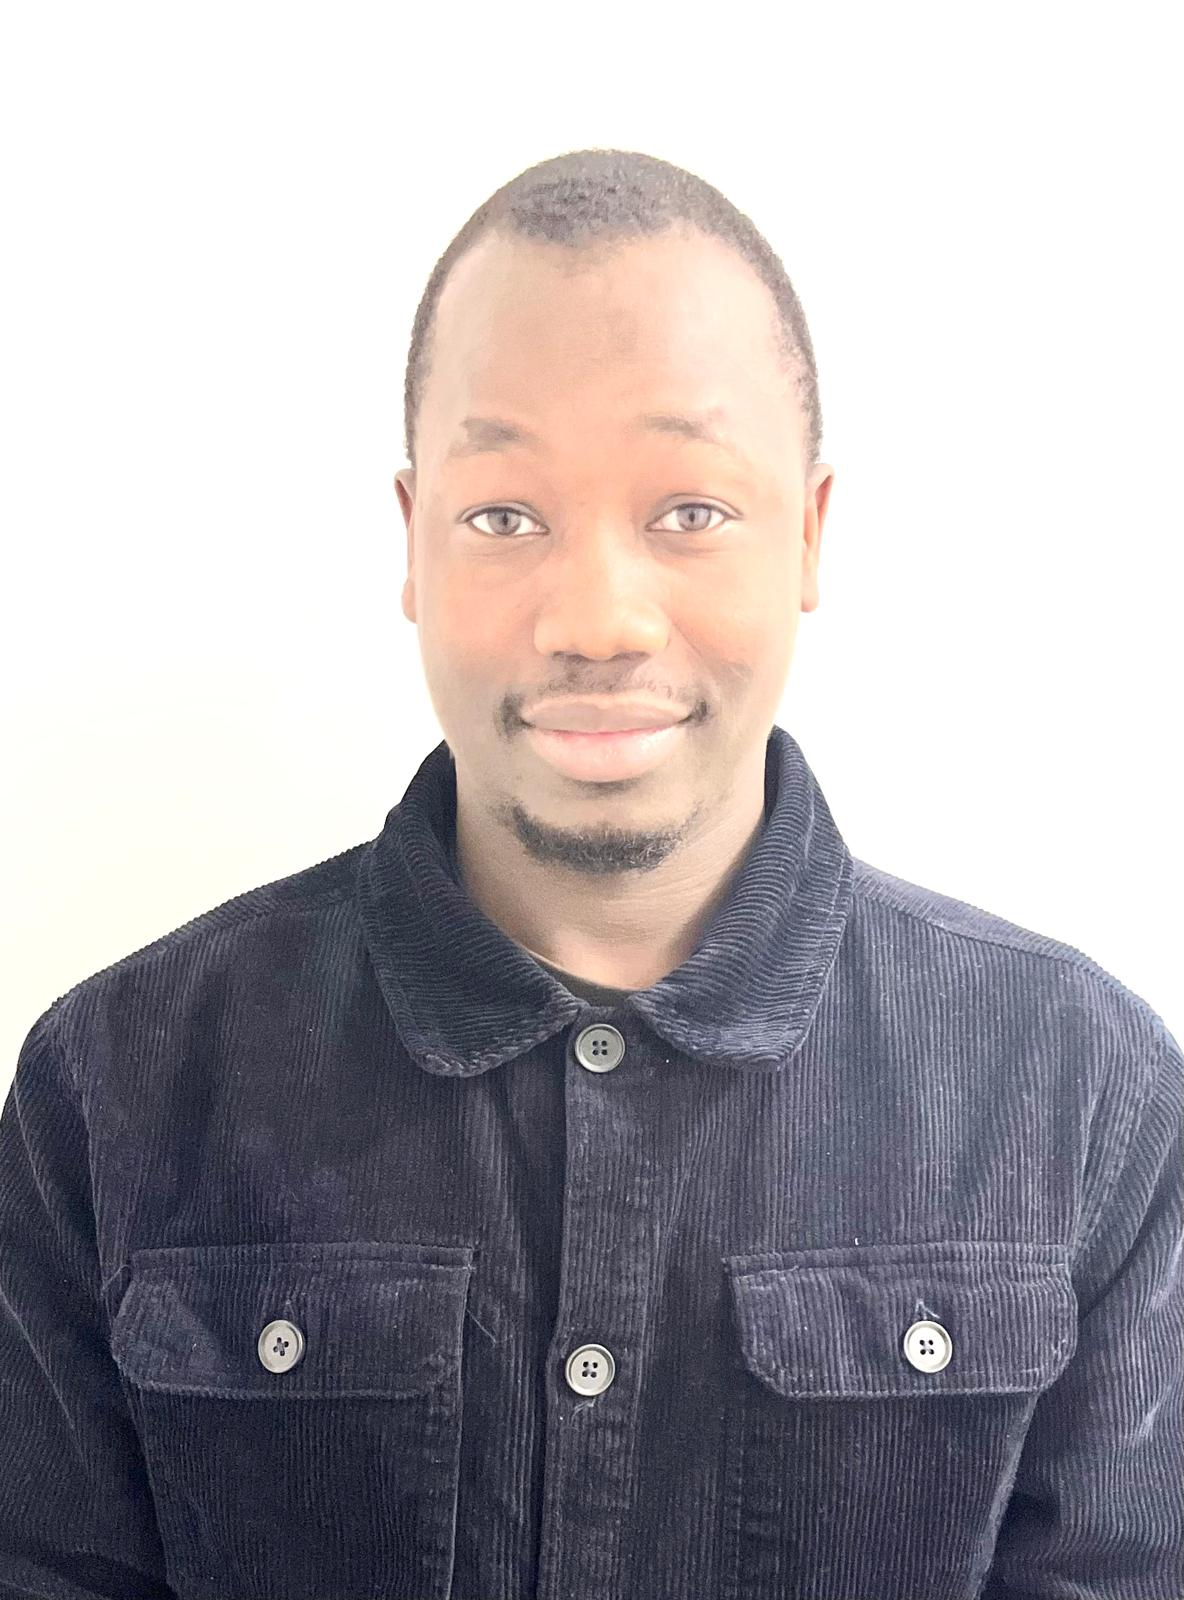
\includegraphics[width=3cm]{d636a17c9cf6472988ce2da23437bf5d.jpg}};
  \end{tikzpicture}
  \fi

  \vspace{3mm}
  {\color{black}\LARGE \textbf{Pape Saliou FALL}}

  \vspace{1mm}
  {\large Ingénieur Data Scientist et Développeur IA}

  \vspace{3mm}
  {\color{gray}\rule{\linewidth}{0.4pt}} \\
\end{minipage}

% ── Coordonnées
\begin{tabular}{@{}c l}
  \faPhone &
  \begin{tabular}[t]{@{}l@{}}
    {\color{gray}Téléphone} \\ 0753481453
  \end{tabular} \\
  \\
  \faLinkedin &
  \begin{tabular}[t]{@{}l@{}}
    {\color{gray}LinkedIn} \\
    \href{@pape-saliou-fall-43154a211/}{}
  \end{tabular} \\
  \\
  \faMapMarker &
  \begin{tabular}[t]{@{}l@{}}
    {\color{gray}Adresse} \\ 95300 Pontoise \\ 
  \end{tabular} \\
  \\
  \faEnvelope &
  \begin{tabular}[t]{@{}l@{}}
    {\color{gray}Email} \\
    \href{mailto:papesalioufall2@gmail.com}{papesalioufall2@gmail.com}
  \end{tabular} \\
\end{tabular}

\vspace{2mm}
{\color{gray}\rule{\linewidth}{0.4pt}} \\

% ── Langues --------------------------------------------------------
{\color{black}{Langues}}

\vspace{2mm}
\begin{itemize}[leftmargin=*]
\item Français - \textcolor{gray}{Natif}
\item Anglais - \textcolor{gray}{B2}\end{itemize}          % ← le placeholder va contenir \begin{itemize}…\end{itemize}
\vspace{2mm}
{\color{gray}\rule{\linewidth}{0.4pt}} \\

% ── Compétences ----------------------------------------------------
\vspace{2mm}
{\color{black}{Compétences Clés}}

\vspace{2mm}
\begin{itemize}[leftmargin=*]
\item Python
\item SQL
\item Tensorflow
\item Scikit-learn
\item PowerBI
\item Git
\item Flask\end{itemize}              % ← idem, une vraie liste
\vspace{2mm}
{\color{gray}\rule{\linewidth}{0.4pt}} \\

% ── Centres d'intérêt
\vspace{2mm}
{\color{black}{Centres d’intérêt}}

\vspace{2mm}
\begin{itemize}[leftmargin=*]
\item Football
\item Natation
\item Lecture
\end{itemize}     % ← simple itemize ou tabular

\vfill
~

% ────────────────────────────────────────
\switchcolumn
% Colonne droite
% ────────────────────────────────────────
\color{black}

% ── Profil
\textcolor{black}{\Large \textbf{Profil Professionnel}} \\[2pt]
Data scientist en CDI, je transforme des ensembles de données complexes en solutions d’IA robustes et évolutives. Autonome et proactif, j’ai conçu des plateformes, des modèles prédictifs et des tableaux de bord qui accélèrent la prise de décision. Passionné par l’innovation, je souhaite rejoindre une organisation ambitieuse pour mettre à profit mes compétences en machine learning et en développement applicatif. \\[8pt]

% ── Expérience
\textcolor{black}{\Large \textbf{Expérience Professionnelle}} \\[2pt]
\colorbox{maincolor}{%
  \begin{minipage}{\linewidth}
    \noindent
    \textbf{Data Scientist \& Développeur IA}\hfill depuis 01/2024\\
    Prepaya\\[-0.3em]
    \begin{itemize}[leftmargin=*]
      \item Conçu et déployé une plateforme IA full-stack (Python/JavaScript, Flask, TensorFlow) sur Heroku. \item Développé des modèles de machine learning et de prévision temporelle connectés à PostgreSQL pour l’analyse des données clients. \item Intégré l’API OpenAI et automatisé le pipeline CI/CD, divisant par deux le délai de mise en production.
    \end{itemize}
  \end{minipage}}

\vspace{3mm}

\colorbox{maincolor}{%
  \begin{minipage}{\linewidth}
    \noindent
    \textbf{Apprenti Risk Analyst \& Data Scientist}\hfill 12/2022 - 12/2023\\
    AXA XL (Groupe AXA)\\[-0.3em]
    \begin{itemize}[leftmargin=*]
      \item Automatisé la collecte de données financières (Python, VBA, SQL), supprimant les tâches manuelles répétitives. \item Construit des tableaux de bord Power BI pour le suivi de la facturation et le reporting à la direction financière. \item Mis au point des modèles prédictifs permettant d’estimer la probabilité de sinistre par client.
    \end{itemize}
  \end{minipage}}

\vspace{3mm}

\colorbox{maincolor}{%
  \begin{minipage}{\linewidth}
    \noindent
    \textbf{Apprenti Data Scientist}\hfill 09/2021 - 08/2022\\
    Prepaya\\[-0.3em]
    \begin{itemize}[leftmargin=*]
      \item Déployé des modèles NLP (BERT, T5) afin de générer automatiquement des formulaires structurés. \item Réalisé une analyse de sentiment des retours clients pour identifier les axes d’amélioration. \item Industrialisé la collecte et le pré-traitement de données web (BeautifulSoup, Selenium).
    \end{itemize}
  \end{minipage}}   % ← blocs \colorbox{maincolor}{\begin{minipage}…}

\vspace{8mm}

% ── Formation
\textcolor{black}{\Large \textbf{Formation}} \\[2pt]
\colorbox{maincolor}{%
  \begin{minipage}{\linewidth}
    \noindent
    \textbf{Master 2 Data Science}\hfill 09/2021 - 03/2022\\
    Sorbonne Université\\[-0.3em]
    \begin{itemize}[leftmargin=*]
      \item Machine learning avancé, deep learning et séries chronologiques. \item Statistiques, bases de données et data visualisation. \item Programmation Python/R et calcul parallèle.
    \end{itemize}
  \end{minipage}}       % ← lignes tabular par diplôme

\end{paracol}
\end{document}

